% Project Management Plan Documentation Template %
% Template made following ISO/IEC/IEEE 16326:2009 %

% Author : Alejandro Muñoz Del Álamo %
% Copyright 2019 %

% Project Basic Concepts File %

\chapter{Antecedentes}
\thispagestyle{chapterpage}

\section{Estado del Arte}
% No se habla del estado actual de la tecnología con la 
% que se desarrollará el trabajo, sino de qué otras 
% aplicaciones existen actualmente o han existido en el 
% mercado (historia de la evolución tecnológica) y que
% realicen funcionalidades iguales o parecidas a las que 
% se propone desarrollar en el TFG.

\subsection{Situación actual de la tecnología}
Con el objetivo de simplificar el proceso de creación de 
personajes en los juegos de rol tradicionales, se han originado 
multitud de aplicaciones con diferentes funciones y finalidades.

Algunas de las aplicaciones son referencias completas de 
los juegos, que sirven como elementos de consulta accesibles, 
rápidos y precisos. Un ejemplo de ello es \textit{\textbf{5e Character}},
que es una referencia completa de personajes para \textit{Dragones y 
Mazmorras, 5ª Edición}.\bigskip
% https://play.google.com/store/apps/details?id=com.dungeon.dev.a5echaracter&hl=en_US

\begin{figure}[H]
    \centering
    \begin{minipage}{0.38\textwidth}
        \centering
        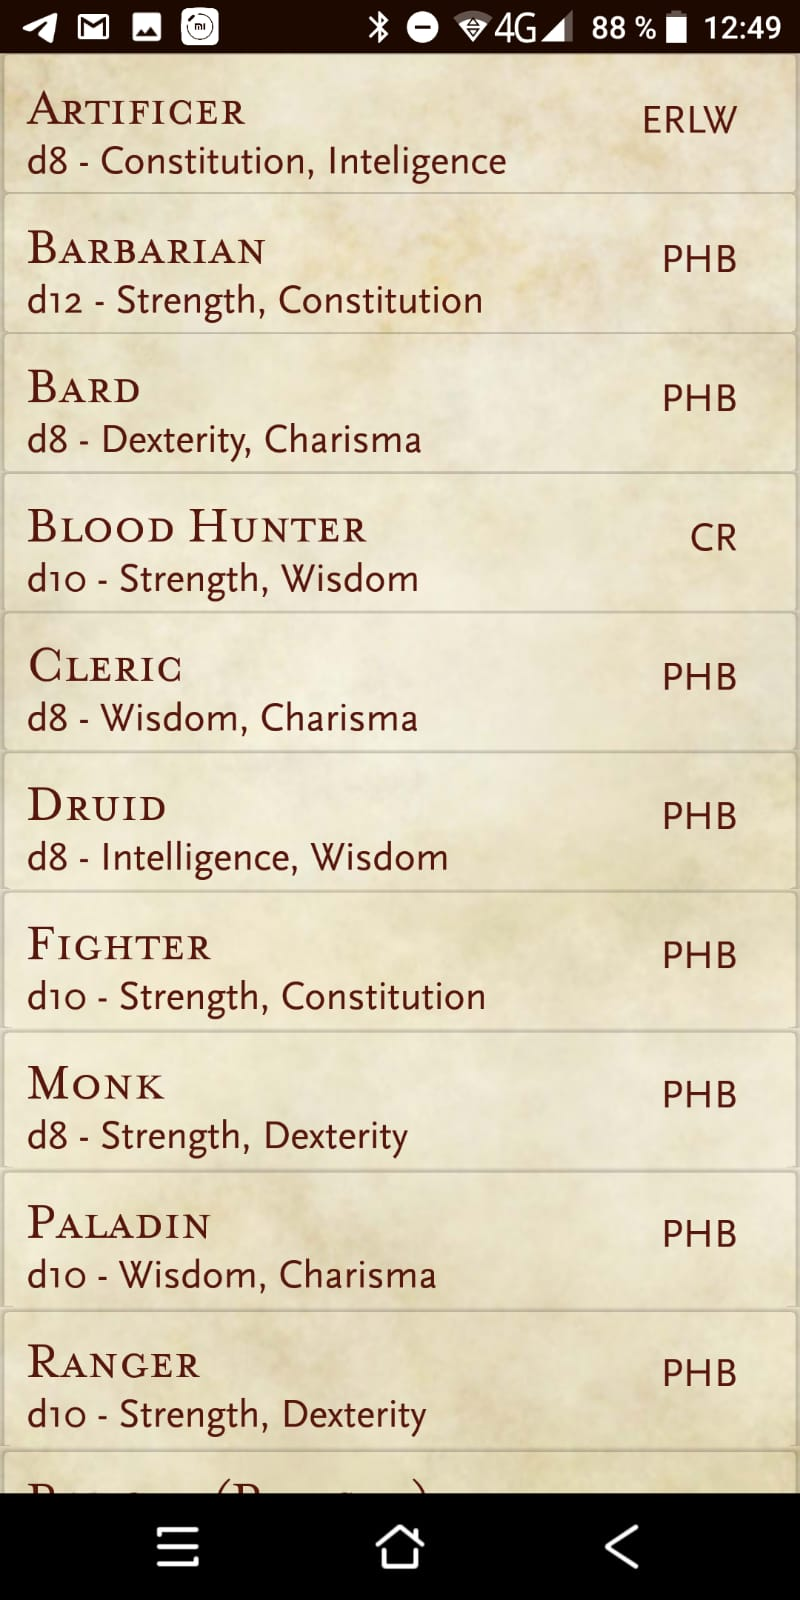
\includegraphics[width=0.5\textwidth]{Images/5e_Character_1.jpeg}
        \caption{\textit{\textbf{5e Character}}: Pantalla de selección 
        de clases}
        
    \end{minipage} \hspace{2cm}
    \begin{minipage}{0.38\textwidth}
        \centering
        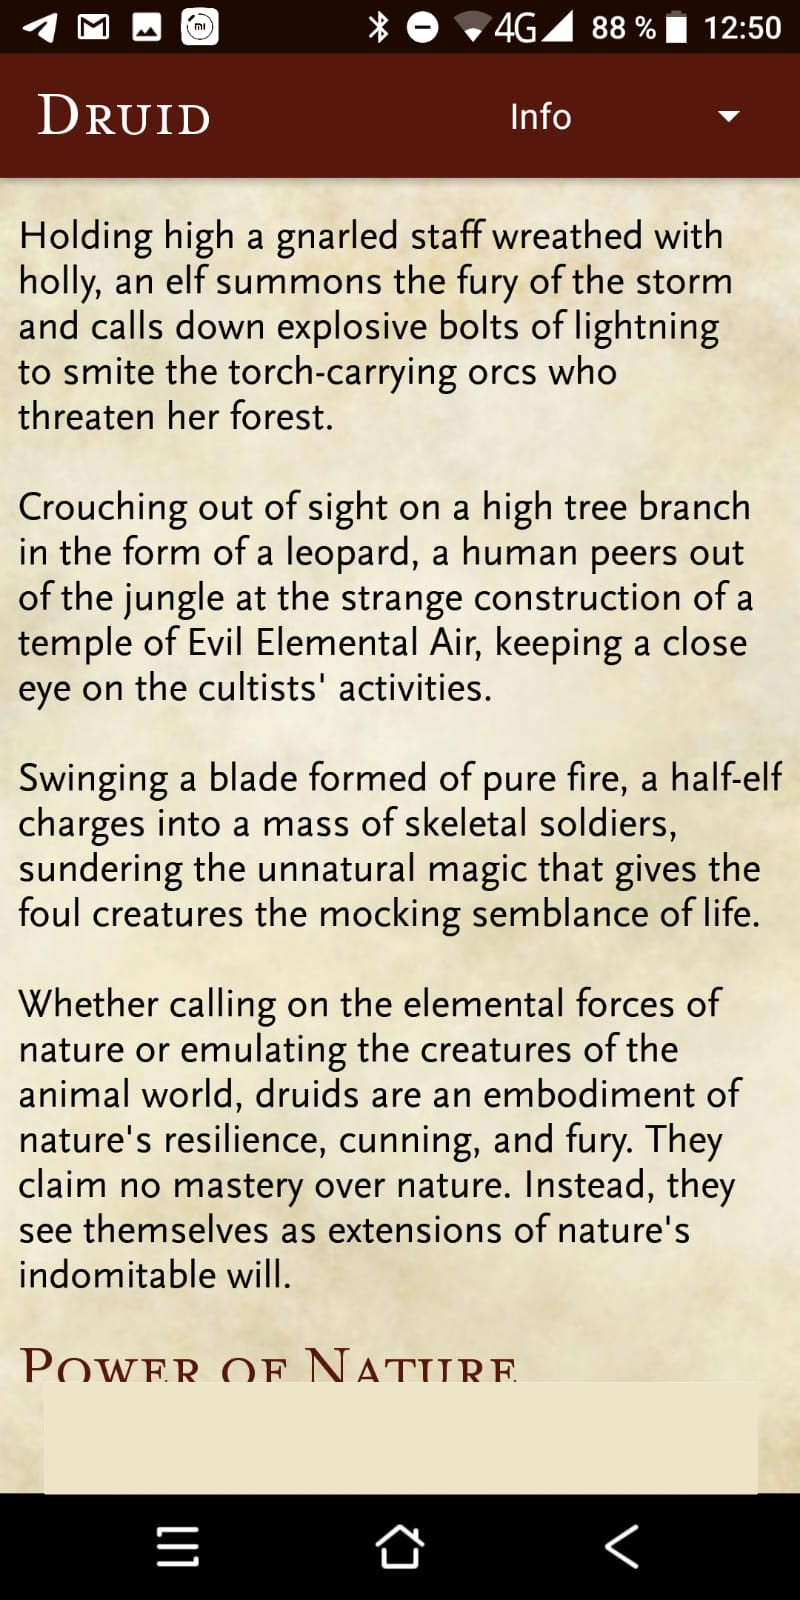
\includegraphics[width=0.5\textwidth]{Images/5e_Character_2.jpeg}
        \caption{\textit{\textbf{5e Character}}: Información 
        de la clase \textit{Druida}}
        
    \end{minipage}
\end{figure}

También podemos encontrar aplicaciones como \textit{\textbf{RPG Simple Dice}} 
que realizan simulaciones de lanzamiento de dados, en caso de que no 
dispongamos de dados físicos. \bigskip

\begin{figure}[H]
    \centering
    \begin{minipage}{0.35\textwidth}
        \centering
        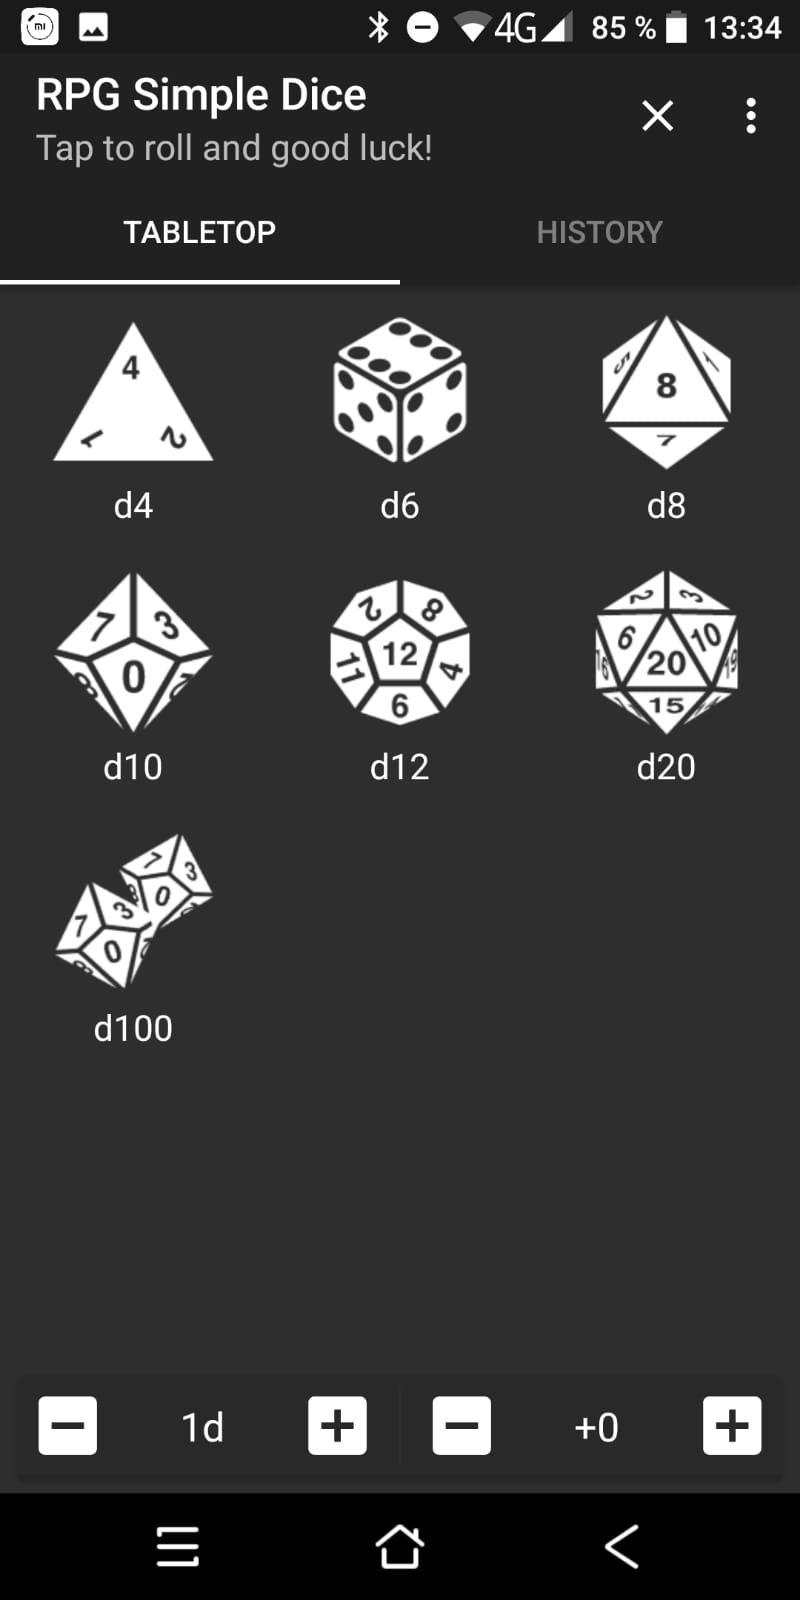
\includegraphics[width=0.5\textwidth]{Images/RPG_Simple_Dice_1.jpeg}
        \caption{\textit{\textbf{RPG Simple Dice}}: Pantalla de selección 
        de dados}
        
    \end{minipage} \hspace{2cm}
    \begin{minipage}{0.35\textwidth}
        \centering
        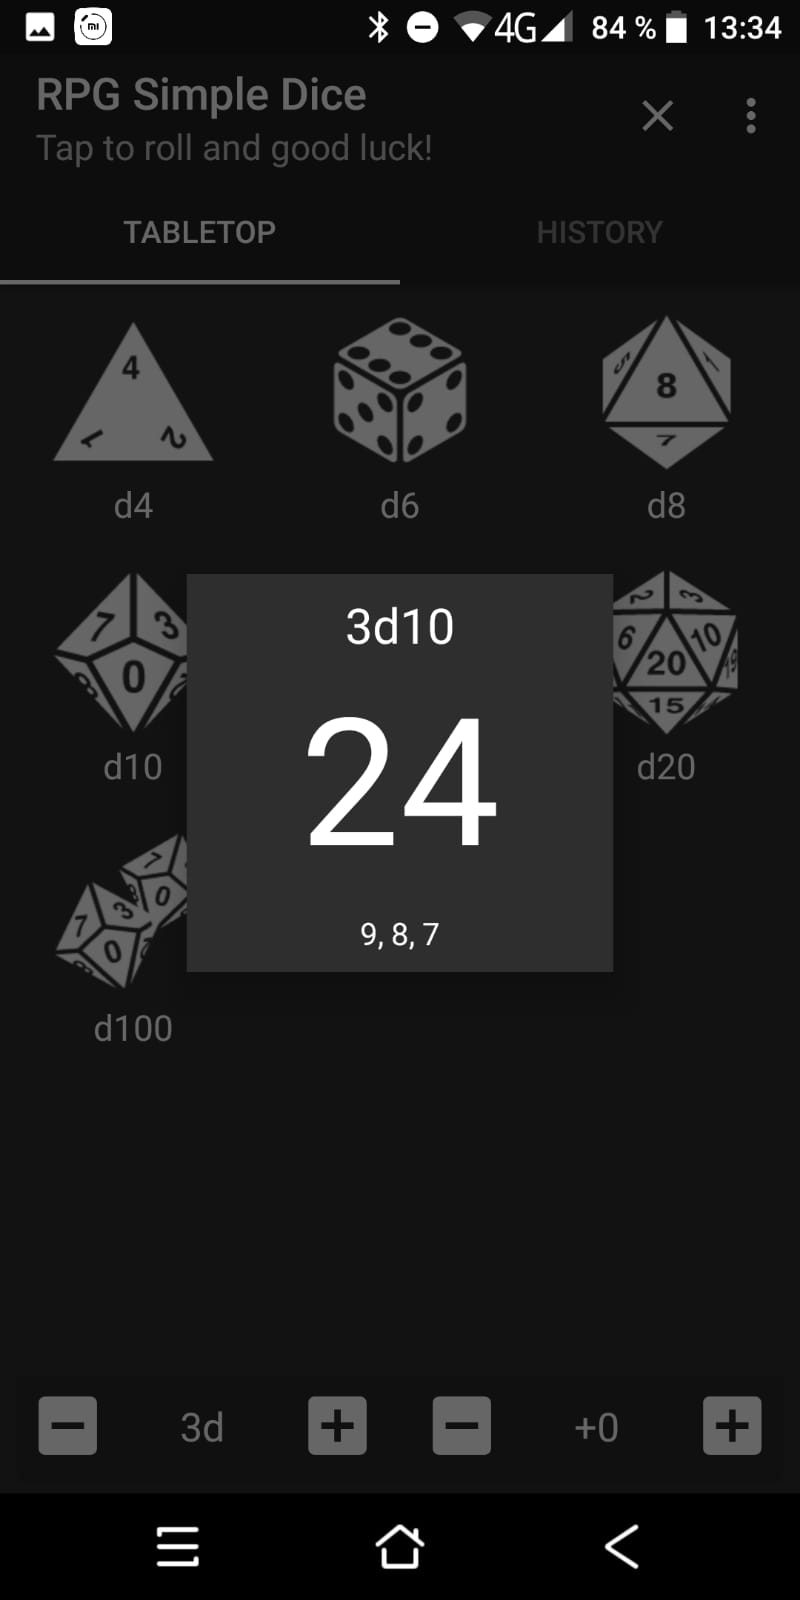
\includegraphics[width=0.5\textwidth]{Images/RPG_Simple_Dice_2.jpeg}
        \caption{\textit{\textbf{RPG Simple Dice}}: Ejemplo de lanzamiento de 
        dados}
        
    \end{minipage}
\end{figure}\bigskip

Otras en cambio, proporcionan algunas herramientas que simplifican algunos 
cálculos que resultan tediosos durante el transcurso de la partida, como 
es el caso de \textit{\textbf{BattleTrack}}. \bigskip

\begin{figure}[H]
    \centering
    \begin{minipage}{0.3\textwidth}
        \centering
        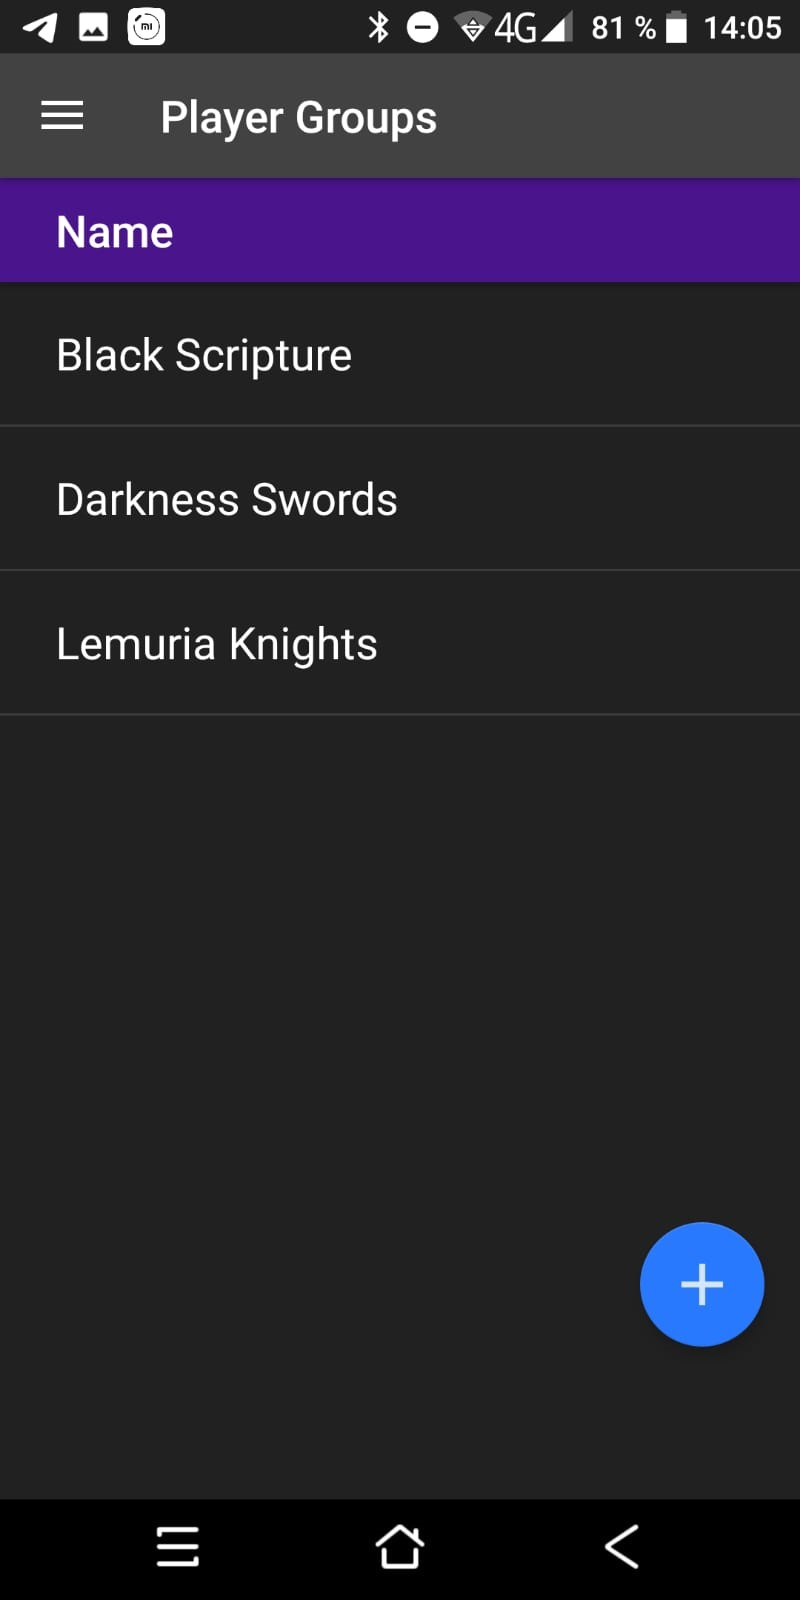
\includegraphics[width=0.7\textwidth]{Images/BattleTrack_1.jpeg}
        \caption{\textit{\textbf{BattleTrack}}: Pantalla de selección 
        de grupo}
        
    \end{minipage} \hspace{2cm}
    \begin{minipage}{0.3\textwidth}
        \centering
        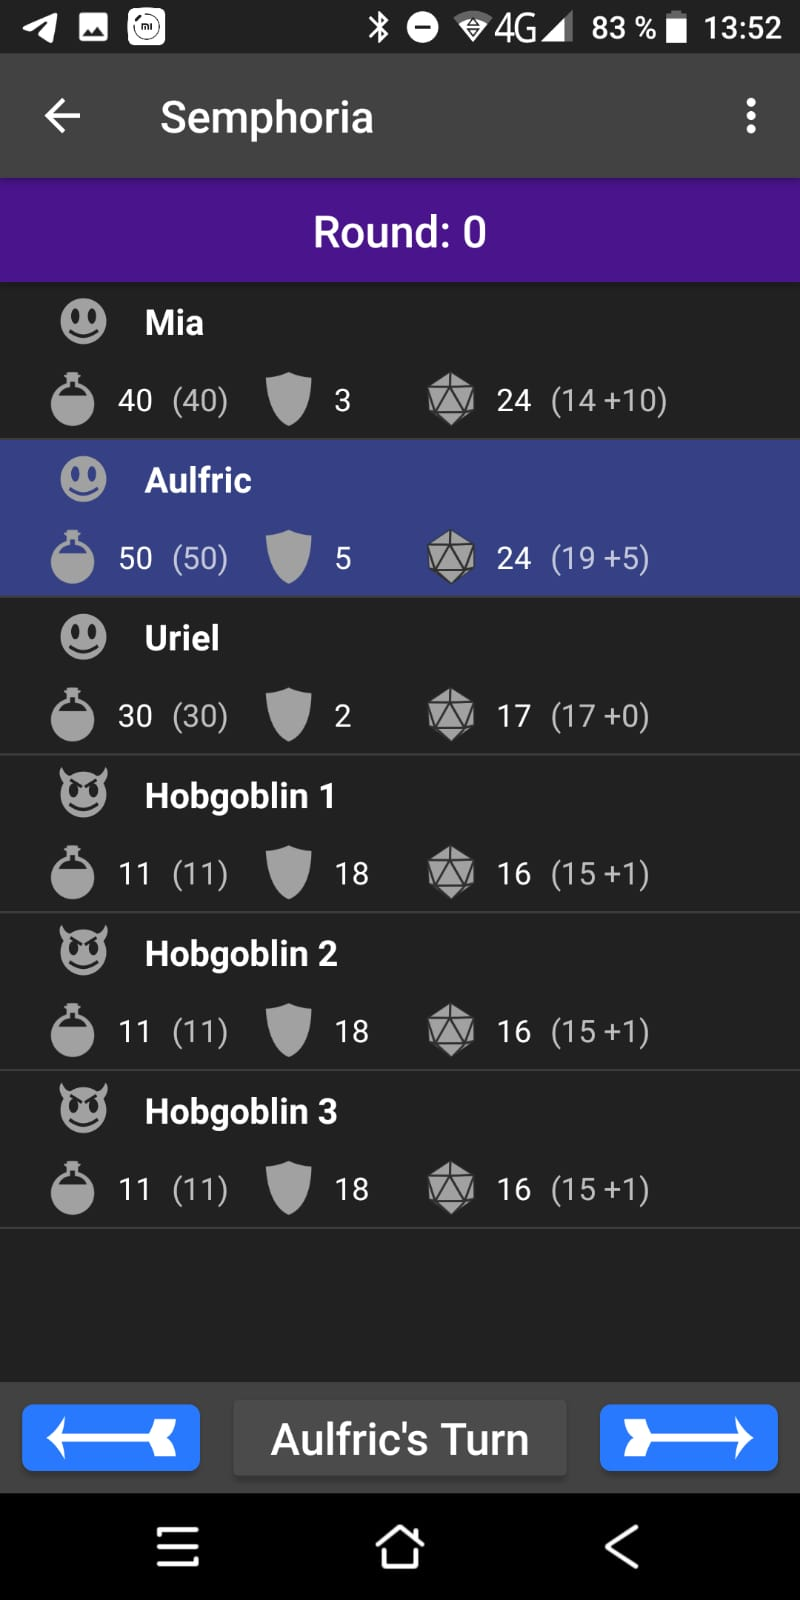
\includegraphics[width=0.7\textwidth]{Images/BattleTrack_2.jpeg}
        \caption{\textit{\textbf{BattleTrack}}: Ejemplo de combate}
        
    \end{minipage}
\end{figure}
\vspace{1cm}

Con el fin de ayudar en la ambientación, aplicaciones como 
\textit{\textbf{RPGSound}} aportan bibliotecas de sonido que se pueden 
utilizar durante la representación de la partida para sumirse en ella.\bigskip

\begin{figure}[H]
    \centering
    \begin{minipage}{0.3\textwidth}
        \centering
        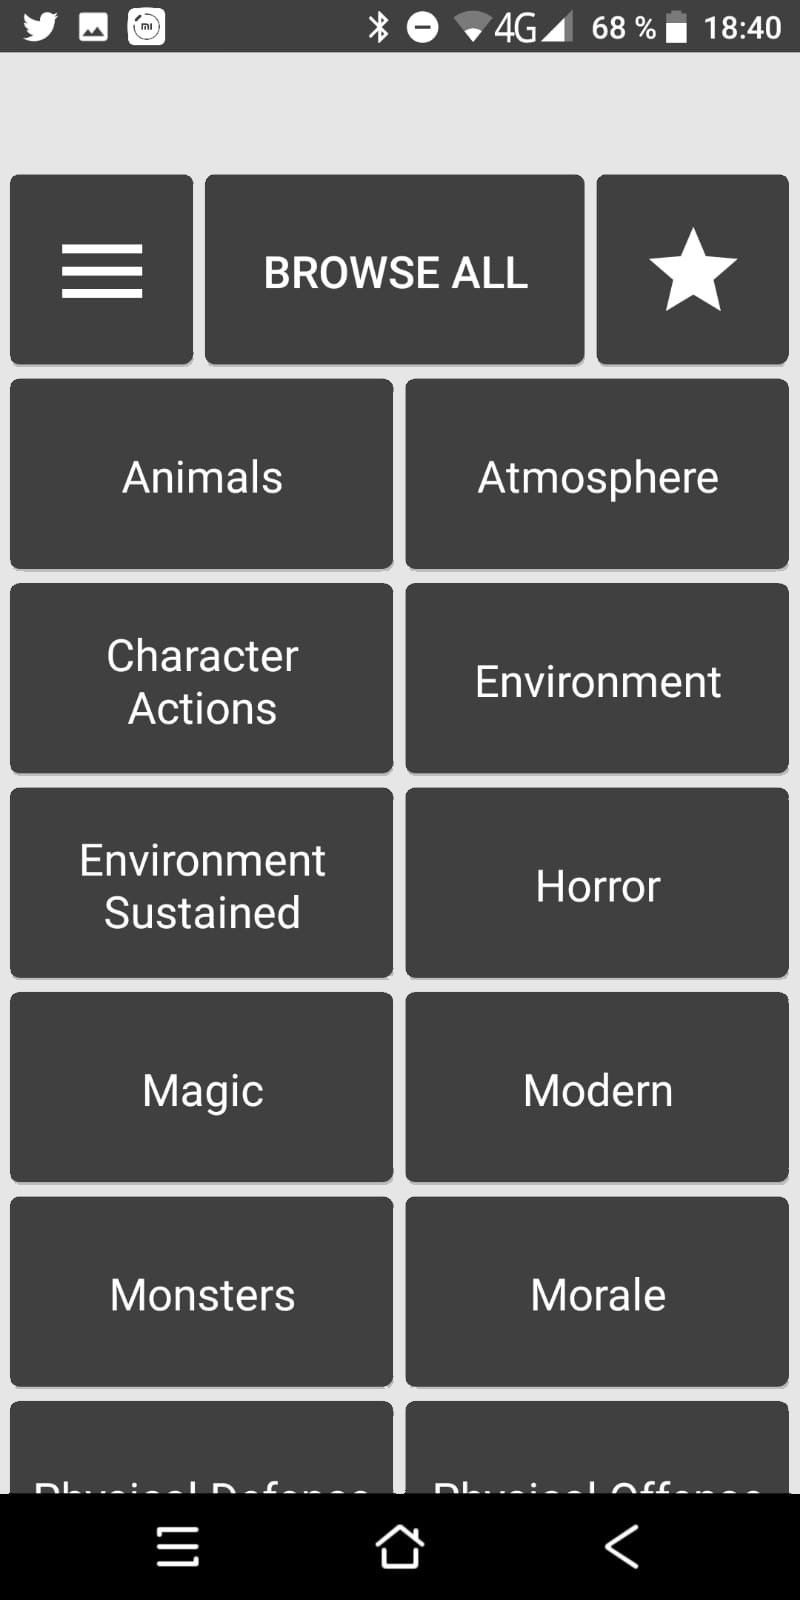
\includegraphics[width=0.7\textwidth]{Images/RPGSound_1.jpeg}
        \caption{\textit{\textbf{RPGSound}}: Menú principal}
        
    \end{minipage} \hspace{2cm}
    \begin{minipage}{0.3\textwidth}
        \centering
        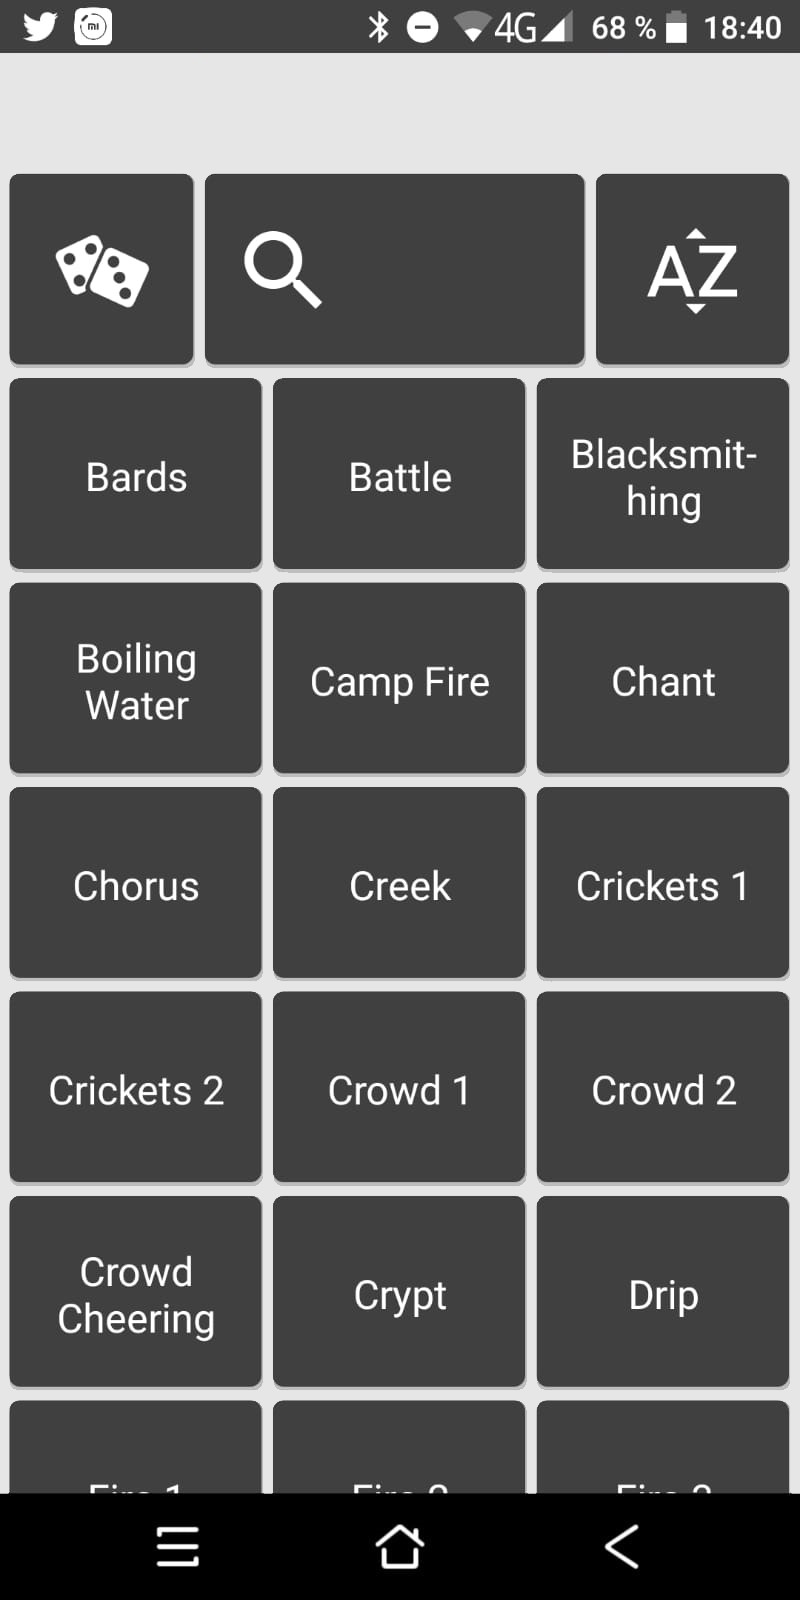
\includegraphics[width=0.7\textwidth]{Images/RPGSound_2.jpeg}
        \caption{\textit{\textbf{RPGSound}}: Menú de \textit{Ambiente 
        Sostenido}}
        
    \end{minipage}
\end{figure}\bigskip

Finalmente, quedan las aplicaciones conocidas como \textit{generadores de
personaje}, que permiten al usuario crear personajes para formar parte de 
una partida de rol, y acceder a esa información de forma rápida. Un buen 
ejemplo de esto es \textit{\textbf{RPG Character Sheet}}.\bigskip

\begin{figure}[H]
    \centering
    \begin{minipage}{0.3\textwidth}
        \centering
        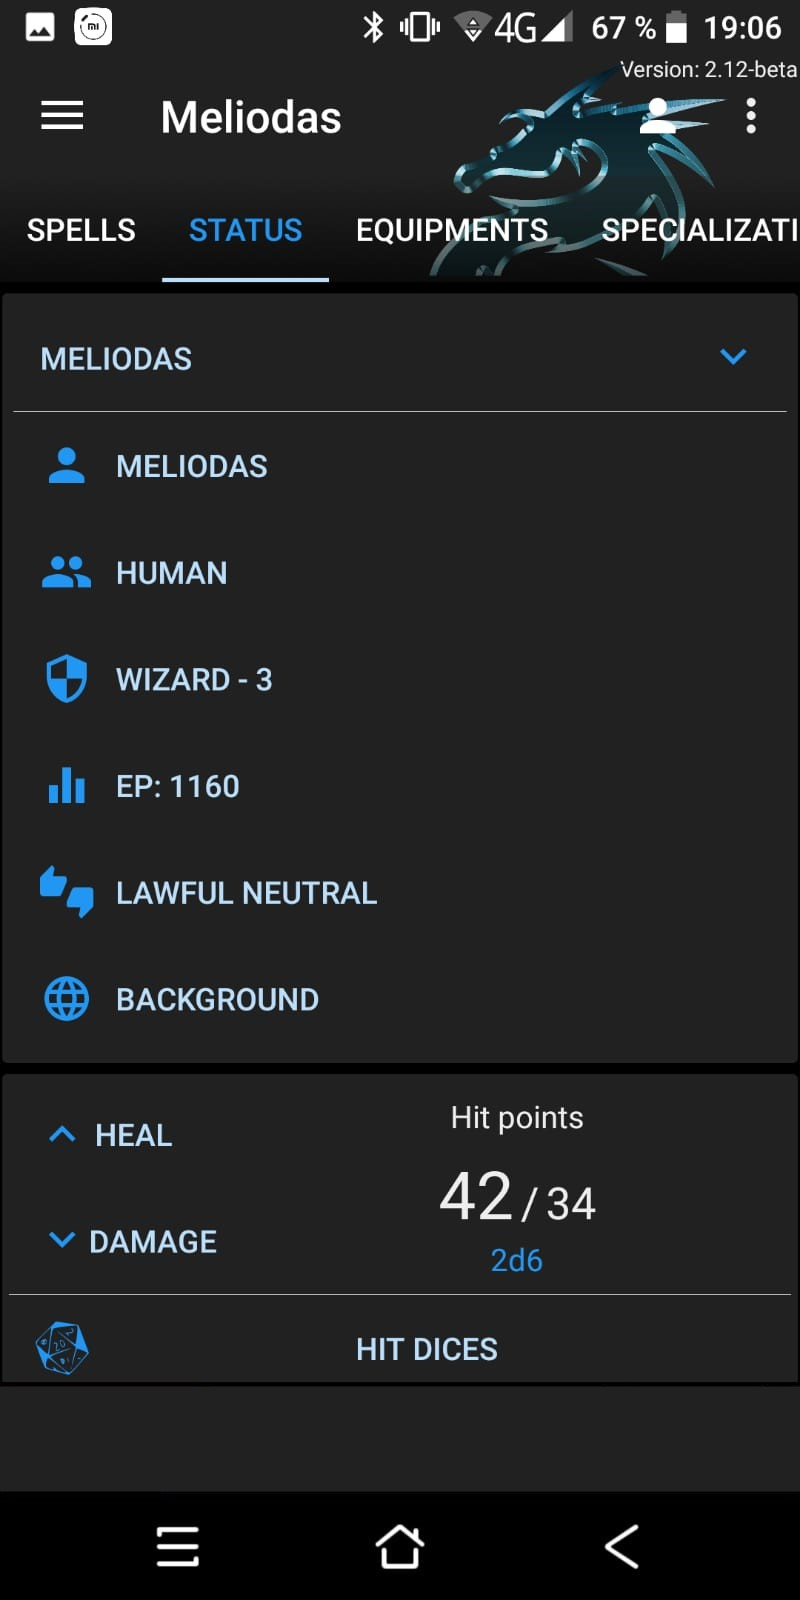
\includegraphics[width=0.7\textwidth]{Images/RPG_Character_Sheet_1.jpeg}
        \caption{\textit{\textbf{RPG Character Sheet}}: Pantalla de \textit{Estado}}
        
    \end{minipage} \hspace{2cm}
    \begin{minipage}{0.3\textwidth}
        \centering
        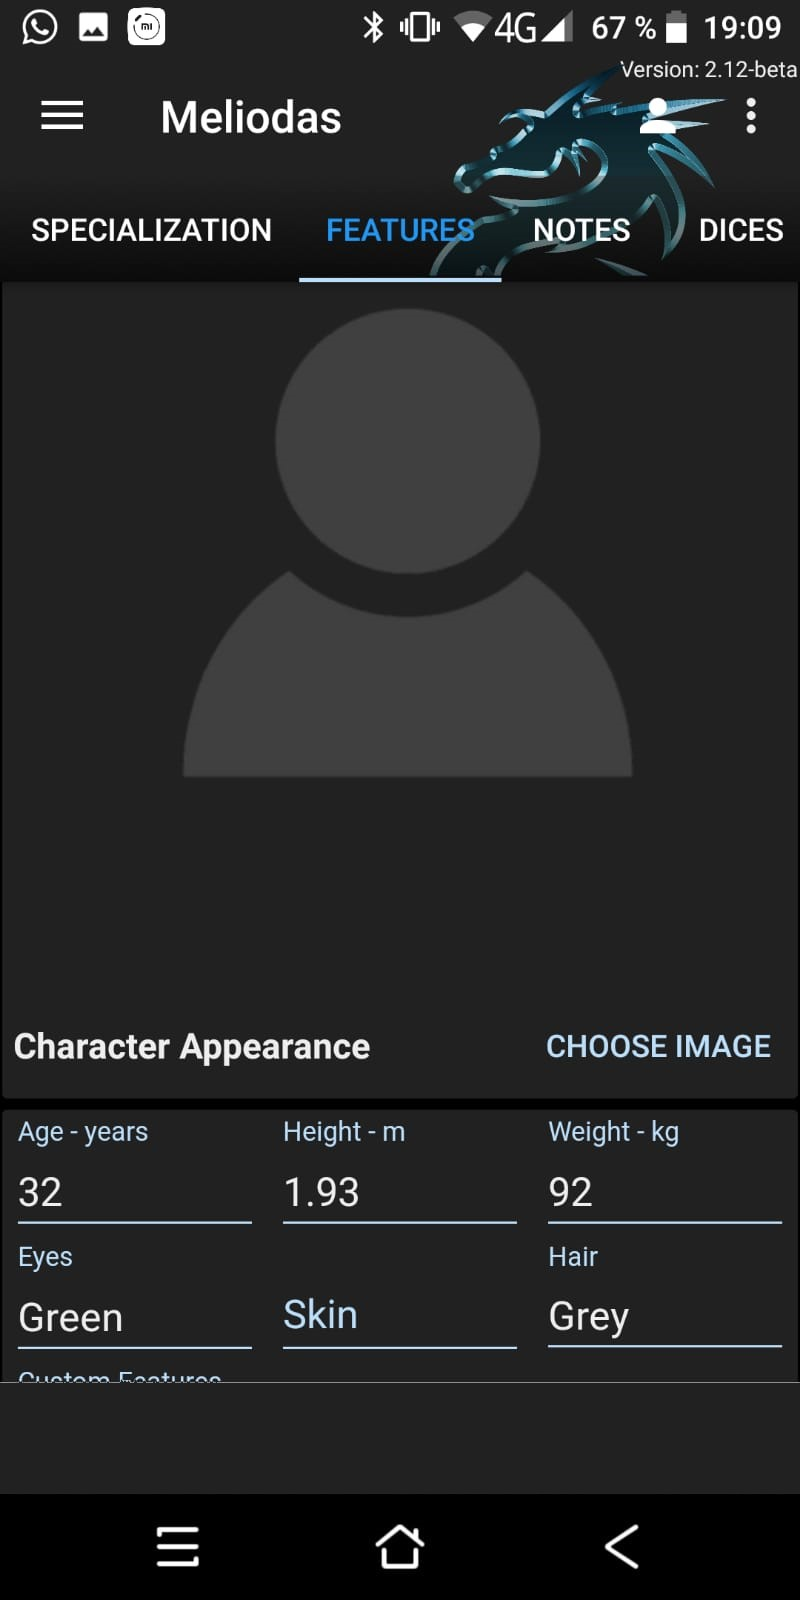
\includegraphics[width=0.7\textwidth]{Images/RPG_Character_Sheet_2.jpeg}
        \caption{\textit{\textbf{RPG Character Sheet}}: Pantalla de 
        \textit{Features}}
        
    \end{minipage}
\end{figure}

% En esta parte donde se concentrarán el 90% de las 
% referencias bibliográficas que aparezcan alfinal 
% de la memoria.

\subsection{Crítica al estado del arte}
Tal y como se ha comentado previamente, existe un holgado abanico de 
aplicaciones cuya meta es mejorar y/o simplificar aspectos en lo referente a 
los juegos de rol, y aunque cumplen con su propósito, a veces no resultan 
tan efectivas como debieran. 
\medskip 

Esto puede deberse a que tras dedicar el tiempo y esfuerzo necesarios para 
desarrollar la aplicación, el estudio del juego ha aprovechado ese tiempo 
de producción para revisar el juego y editarlo, realizando modificaciones 
que provocan que \emph{\textbf{la aplicación quede obsoleta en poco tiempo}}. 
\medskip

Otro inconveniente es que las aplicaciones que requieren mucha información 
específica, como los generadores de personaje, pueden llegar a 
\emph{\textbf{resultar muy complejas}}, provocando que el usuario 
considere que el esfuerzo que tiene que dedicar para aprender cómo utilizarla 
es mayor que el de realizar el proceso manualmente. \medskip

También existen aplicaciones que no contemplan la reutilización de la 
información que han producido para efectuar operaciones que mejoren 
la jugabilidad, por lo que el usuario no le ve provecho a emplear dichas
aplicaciones.

\subsection{Propuesta}
Tomando en consideración los aspectos comentados en el apartado anterior, 
se ha formulado la siguiente solución:
\begin{itemize}
    \item La aplicación permitirá al usuario seleccionar en qué juego y 
    versión desea que trabaje la aplicación.
    \item La aplicación distribuirá el proceso de creación de personajes del 
    juego seleccionado en un conjunto modular secuenciado de pasos a seguir, 
    que guíe al usuario en el proceso y resulte sencillo de utilizar. 
    \item La aplicación tendrá la capacidad de reutilizar los datos 
    producidos para operar con ellos, ofreciendo al usuario información 
    adicional práctica para algunos aspectos del juego escogido.
\end{itemize}





